\documentclass[10pt,aspectratio=169]{beamer}

\usetheme{metropolis}
\usepackage{appendixnumberbeamer}
\usepackage{polyglossia}   
\setdefaultlanguage{polish}                         

\usepackage{booktabs}
\usepackage[scale=2]{ccicons}

\usepackage{pgfplots}
\usepgfplotslibrary{dateplot}

\usepackage{xspace}
\usepackage{subcaption}
\captionsetup[sub]{font=tiny}
\newcommand{\themename}{\textbf{\textsc{metropolis}}\xspace}
\setbeamercolor{background canvas}{bg=white}

\newcommand{\img}[3]
{
  \begin{figure}
    \centering
        \includegraphics[width=#2,height=#3,keepaspectratio]{obrazy/#1}
  \end{figure}
}

\title{Algorytmy poleceń mentalnych w interfejsach mózg--komputer}
%\subtitle{Algorithms of mental commands in brain-computer interfaces}
\date{} %\date{\today}
\author{Adam Baniuszewicz\\Teleinformatyka S2}
\institute{Promotor: dr inż. Robert Krupiński\\
Katedra Przetwarzania Sygnałów i Inżynierii Multimedialnej\\
Wydział Elektryczny ZUT w Szczecinie}
% \titlegraphic{\hfill\includegraphics[height=1.5cm]{logo.pdf}}

\begin{document}

\maketitle

\begin{frame}{Spis treści}
  \setbeamertemplate{section in toc}[sections numbered]
  \tableofcontents[hideallsubsections]
\end{frame}

\section{Cel i zakres pracy}

\begin{frame}{Cel pracy}
  Wykonanie układu wirtualnej klawiatury sterowanej przy użyciu urządzenia do rejestracji aktywności mózgu.
\end{frame}

\begin{frame}{Zakres pracy}
  \begin{enumerate}%[<+-|alert@+>]
    \item Analiza urządzeń do rejestracji aktywności mózgu.
    \item Projekt oraz wykonanie układu wirtualnej klawiatury.
    \item Opracowanie algorytmu sterowania wykorzystującego komendy mentalne.
    \item Przeprowadzenie badań opracowanego układu.
  \end{enumerate}
\end{frame}

\section{Wstęp do tematyki interfejsów mózg--komputer}

\begin{frame}{Definicja}
  \begin{itemize}[<+->]
    \item[] \alert{Interfejs mózg--komputer} jest układem, który przetwarza aktywność ośrodkowego układu nerwowego w polecenia dla urządzenia wykonawczego.
    \item[] Potencjalne zastosowania: nadzór skupienia, rehabilitacja, gry komputerowe.
  \end{itemize}
\end{frame}

\begin{frame}{Rodzaje interfejsów mózg--komputer}
  \begin{columns}
    \begin{column}{0.4\textwidth}
      \begin{enumerate}[<+-|alert@+>]
        \item Inwazyjne
        \item Nieinwazyjne
      \end{enumerate}
    \end{column}
    \hfill
    \begin{column}{0.6\textwidth}
      \only<1>{\img{invasive}{0.8\linewidth}{0.7\textheight}}
      \only<2>{\img{non_invasive}{0.8\linewidth}{0.7\textheight}}
    \end{column}
  \end{columns}
\end{frame}

\begin{frame}{Podejścia do realizacji sterowania}
  \begin{columns}
    \begin{column}{0.29\textwidth}
      \begin{enumerate}[<+-|alert@+>]
        \item Potencjały wywołane
        \item Wyobrażenie ruchu 
      \end{enumerate}
    \end{column}
    \hfill
    \begin{column}{0.69\textwidth}
      \only<1>{\img{p300}{\linewidth}{0.7\textheight}}
      \only<2>{\img{homunculus}{\linewidth}{0.8\textheight}}
    \end{column}
  \end{columns}
\end{frame}

\section{Charakterystyka wybranych urządzeń komercyjnych}

\begin{frame}{Cechy poszukiwanego urządzenia}
  \begin{enumerate}
    \item Nieinwazyjne
    \item Rozwinięte SDK
    \item Wsparcie w detekcji komend mentalnych
    \item Przystępna cena
  \end{enumerate}
\end{frame}

\begin{frame}{Omówione urządzenia}
  \begin{figure}[htb]
    \centering
    \begin{subfigure}{0.2\linewidth}
    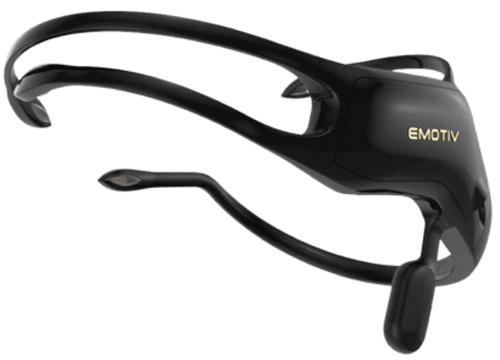
\includegraphics[width=\linewidth,keepaspectratio]{obrazy/insight}
    \caption{Emotiv Insight}
    \end{subfigure}\hspace*{\fill}
    \begin{subfigure}{0.2\linewidth}
    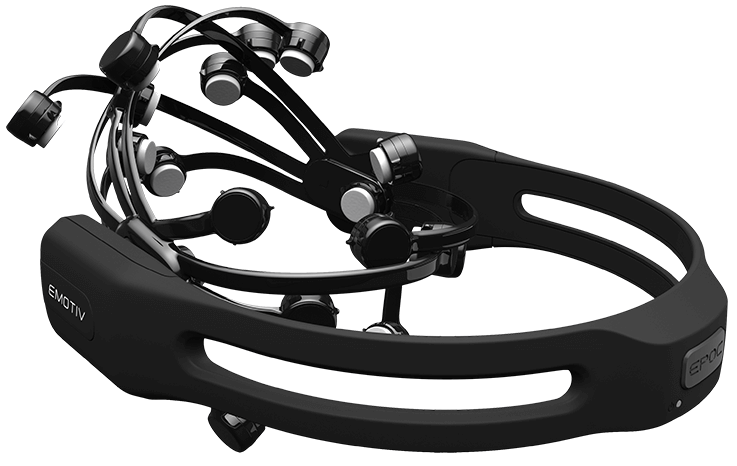
\includegraphics[width=\linewidth,keepaspectratio]{obrazy/epoc}
    \caption{Emotiv EPOC+}
    \end{subfigure}\hspace*{\fill}
    \begin{subfigure}{0.2\linewidth}
    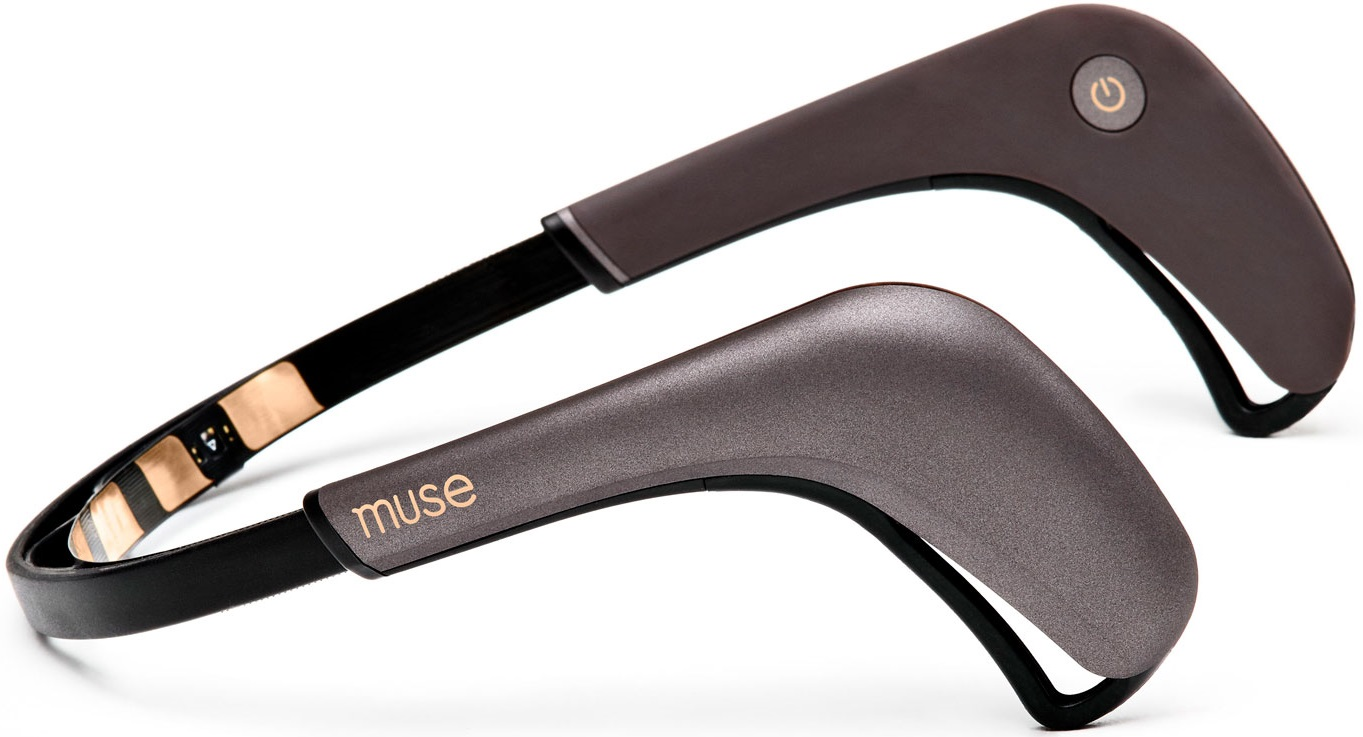
\includegraphics[width=\linewidth,keepaspectratio]{obrazy/muse2}
    \caption{Muse/Muse 2}
    \end{subfigure}
    \par\bigskip
    \hspace*{\fill}\begin{subfigure}{0.2\linewidth}
    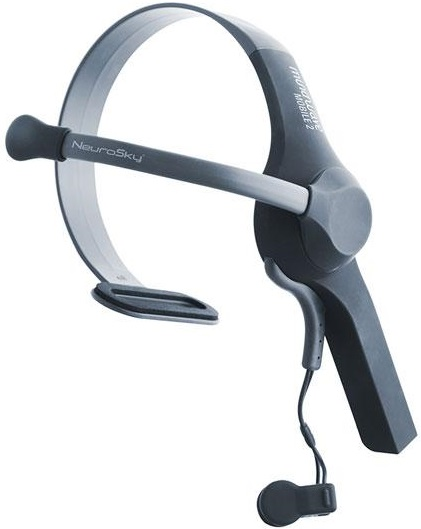
\includegraphics[width=\linewidth,keepaspectratio]{obrazy/mindwave}
    \caption{MindWave Mobile 2}
    \end{subfigure}\hspace*{\fill}
    \begin{subfigure}{0.2\linewidth}
    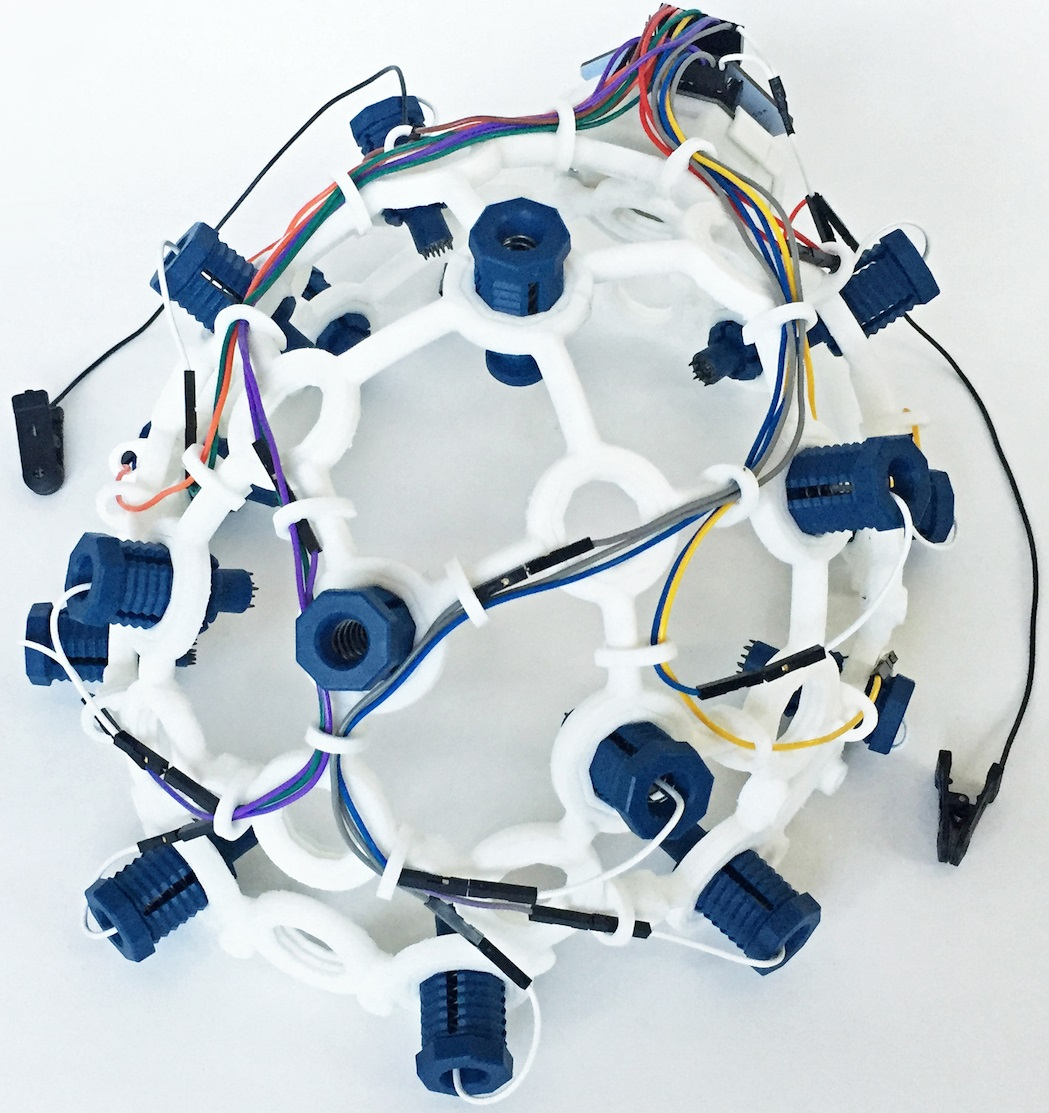
\includegraphics[width=\linewidth,keepaspectratio]{obrazy/markiv}
    \caption{OpenBCI Ultracortex Mark IV}
    \end{subfigure}\hspace*{\fill}
  \end{figure}
\end{frame}

\section{Projekt wirtualnej klawiatury}

\begin{frame}{Wykorzystywane narzędzia}
  \begin{enumerate}
    \item Urządzenie rejestrujące: Emotiv Insight.
    \item Język programowania: C\#.
    \item Środowisko programistyczne: Visual Studio.
    \item System kontroli wersji: Git.
  \end{enumerate}
\end{frame}
\begin{frame}{Trening komend}
  \begin{columns}
    \begin{column}{0.5\textwidth}
      \begin{enumerate}[<+-|alert@+>]
        \item 4 komendy mentalne + 1 mimiczna
        \item Trening detekcji komend mentalnych
        \item Trening detekcji mimiki
      \end{enumerate}
    \end{column}
    \hfill
    \begin{column}{0.5\textwidth}
      \only<2>{\img{emotivbci_left}{0.8\linewidth}{0.7\textheight}}
      \only<3>{\img{facial_frown}{0.8\linewidth}{0.7\textheight}}
    \end{column}
  \end{columns}
\end{frame}
\begin{frame}{Interfejs użytkownika: Virtual Keyboard}
  \img{virtual_keyboard}{\textwidth}{0.8\textheight}
\end{frame}
\begin{frame}{Interfejs użytkownika: Messenger}
  \img{messenger}{\textwidth}{0.8\textheight}
\end{frame}
\begin{frame}{Interfejs użytkownika: Settings}
  \img{settings}{\textwidth}{0.5\textheight}
\end{frame}

\section{Badania opracowanego systemu}
\begin{frame}{Wpływ liczby komend oraz liczby sesji treningowych na poprawność detekcji}
  \begin{figure}[htb]
    \centering
    \begin{subfigure}{0.3\linewidth}
    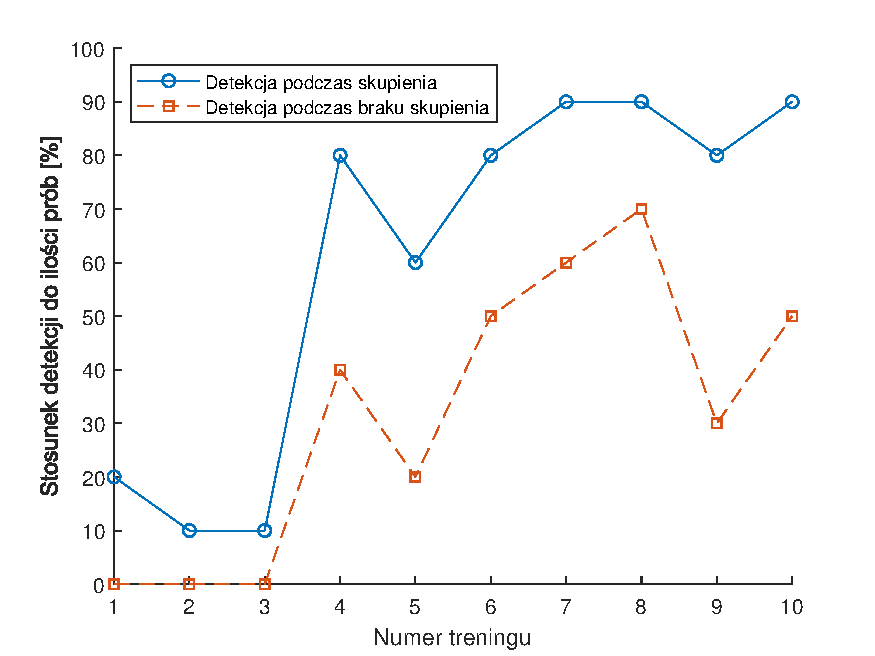
\includegraphics[width=\linewidth,keepaspectratio]{obrazy/up}
    \caption{Uniesienie}
    \end{subfigure}\hspace*{\fill}
    \begin{subfigure}{0.3\linewidth}
    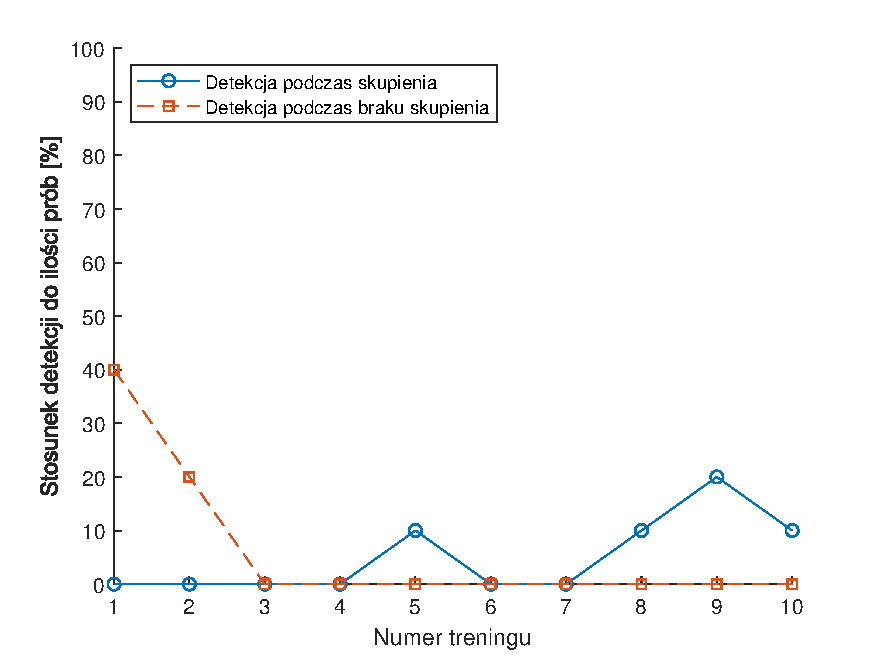
\includegraphics[width=\linewidth,keepaspectratio]{obrazy/right}
    \caption{Przesunięcie w prawo}
    \end{subfigure}\hspace*{\fill}
    \begin{subfigure}{0.3\linewidth}
    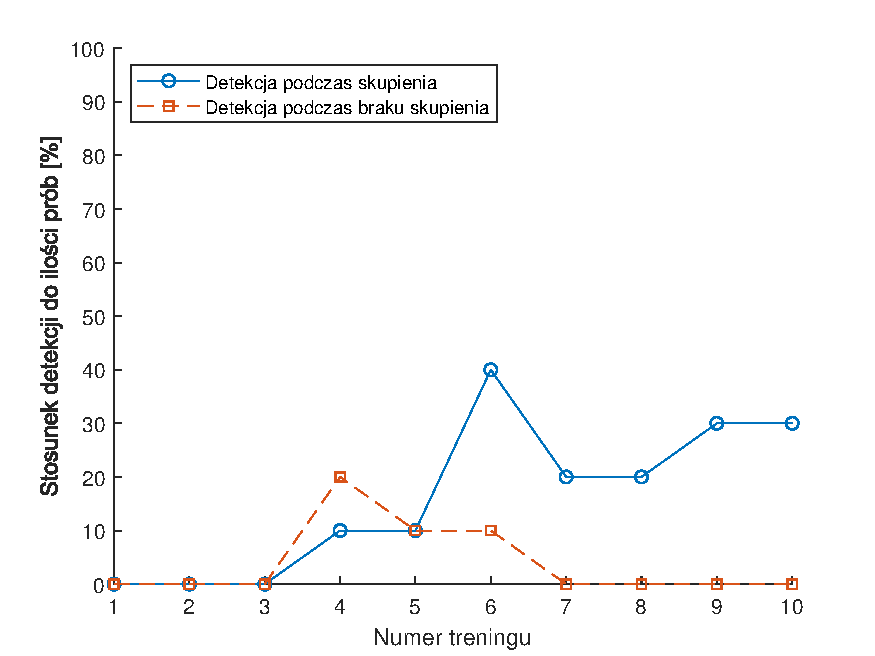
\includegraphics[width=\linewidth,keepaspectratio]{obrazy/down}
    \caption{Opuszczenie}
    \end{subfigure}
    \medskip
    \hspace*{\fill}
    \begin{subfigure}{0.3\linewidth}
    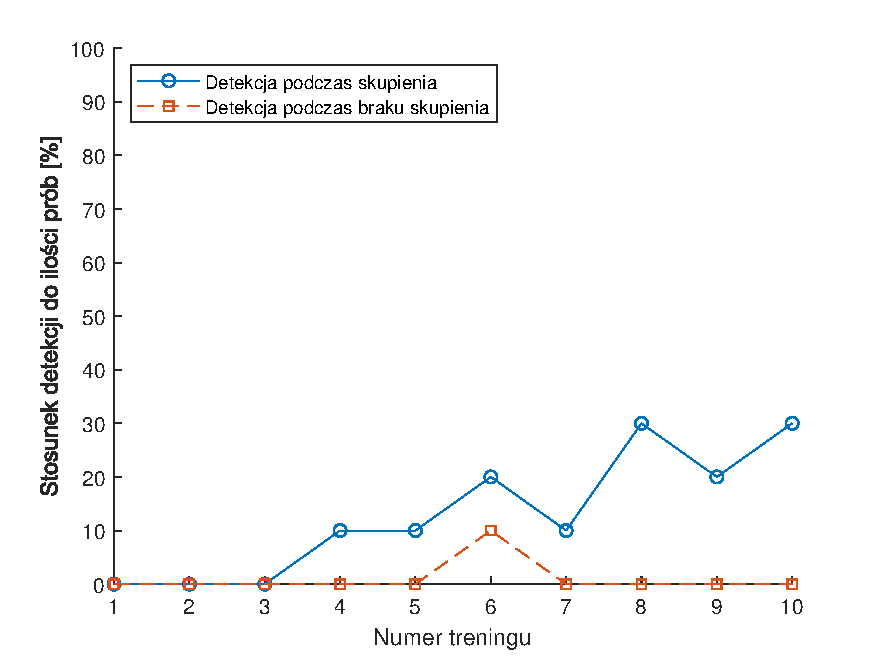
\includegraphics[width=\linewidth,keepaspectratio]{obrazy/left}
    \caption{Przesunięcie w lewo}
    \end{subfigure}\hspace*{\fill}
    \begin{subfigure}{0.3\linewidth}
    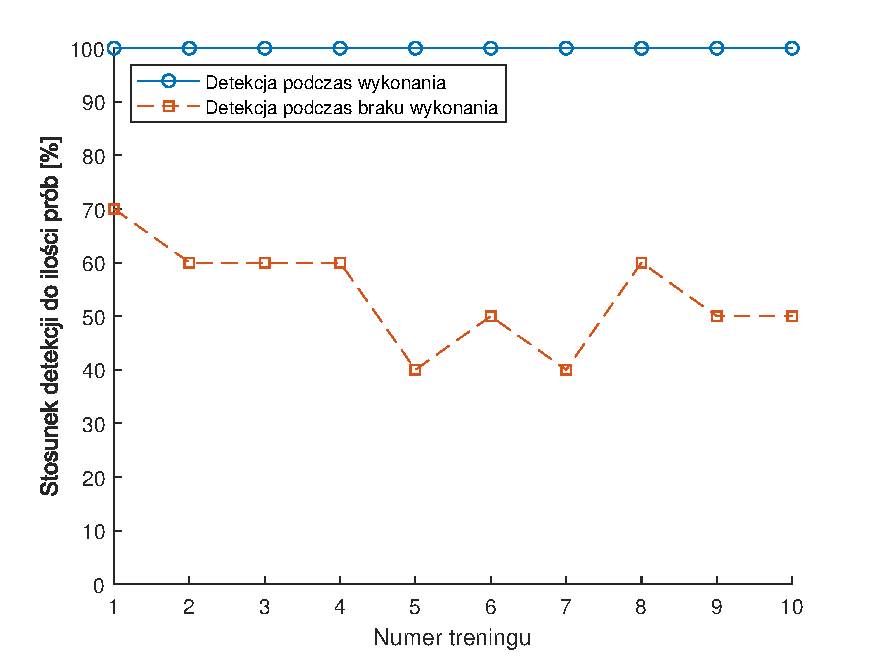
\includegraphics[width=\linewidth,keepaspectratio]{obrazy/frown}
    \caption{Zmarszczenie brwi}
    \end{subfigure}\hspace*{\fill}
  \end{figure}
\end{frame}

\begin{frame}{Wpływ parametrów opracowanej aplikacji na poprawność detekcji}
  \begin{figure}[htb]
    \centering
    \begin{subfigure}{0.3\linewidth}
    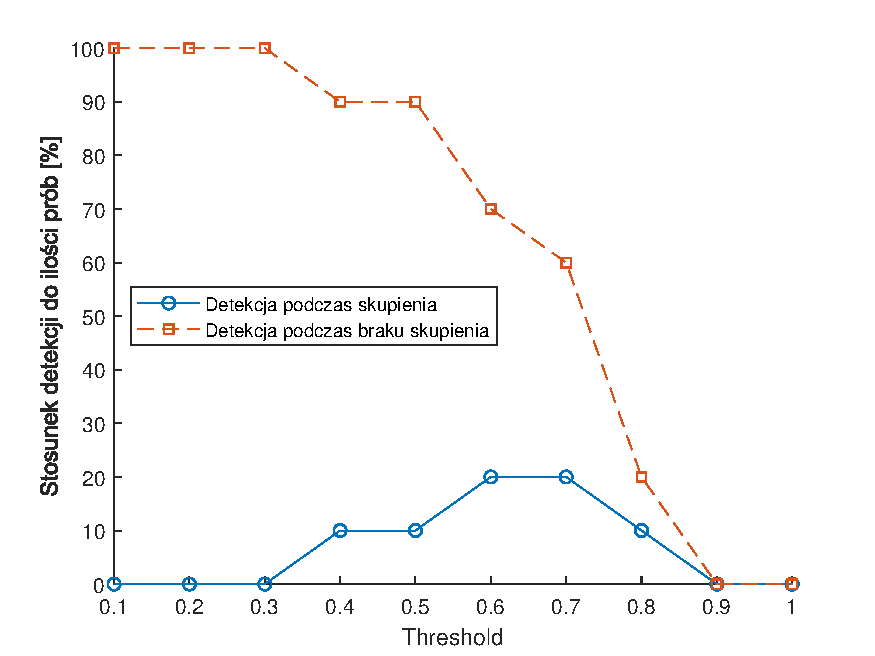
\includegraphics[width=\linewidth,keepaspectratio]{obrazy/up500}
    \caption{Uniesienie, CFT = 500 ms}
    \end{subfigure}\hspace*{\fill}
    \begin{subfigure}{0.3\linewidth}
    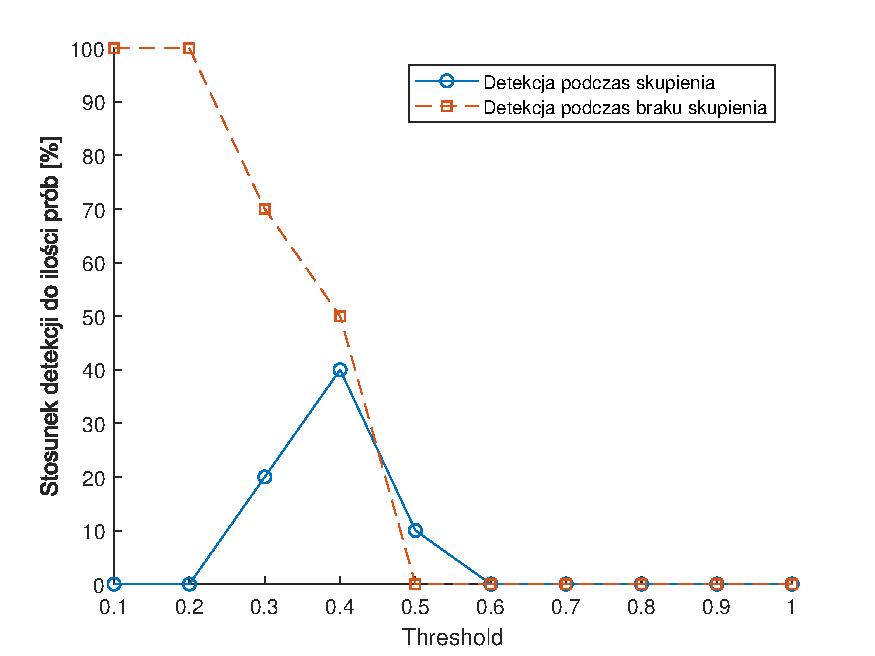
\includegraphics[width=\linewidth,keepaspectratio]{obrazy/up1500}
    \caption{Uniesienie, CFT = 1500 ms}
    \end{subfigure}\hspace*{\fill}
    \begin{subfigure}{0.3\linewidth}
    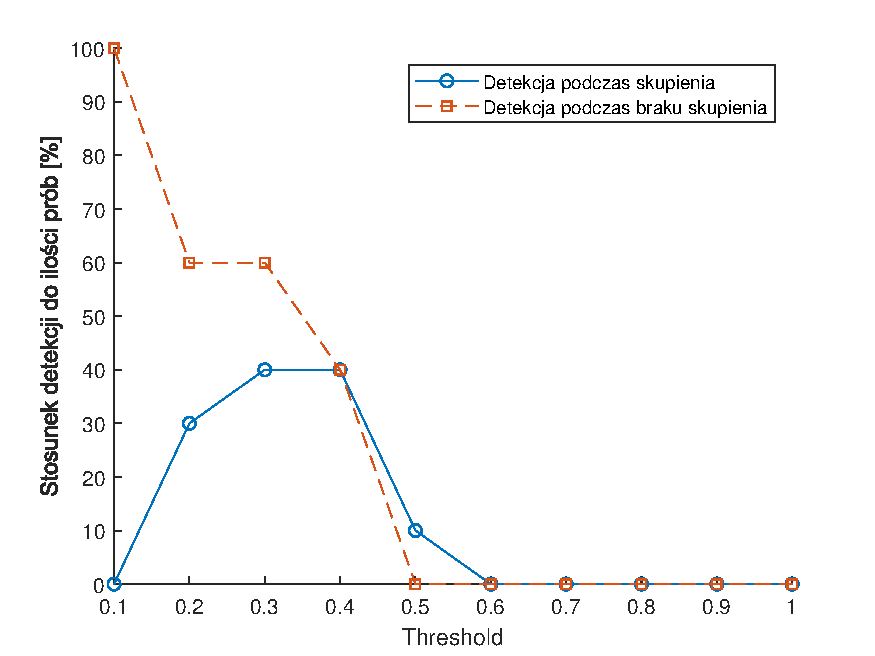
\includegraphics[width=\linewidth,keepaspectratio]{obrazy/up2500}
    \caption{Uniesienie, CFT = 2500 ms}
    \end{subfigure}
    \medskip
    \begin{subfigure}{0.3\linewidth}
    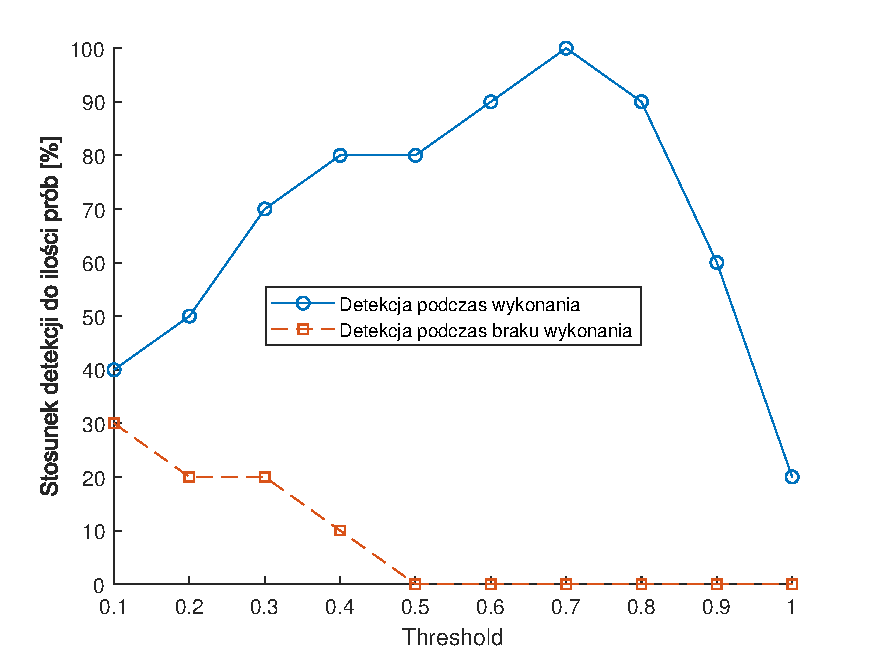
\includegraphics[width=\linewidth,keepaspectratio]{obrazy/frown500}
    \caption{Zmarszczenie brwi, CFT = 500 ms}
    \end{subfigure}\hspace*{\fill}
    \begin{subfigure}{0.3\linewidth}
    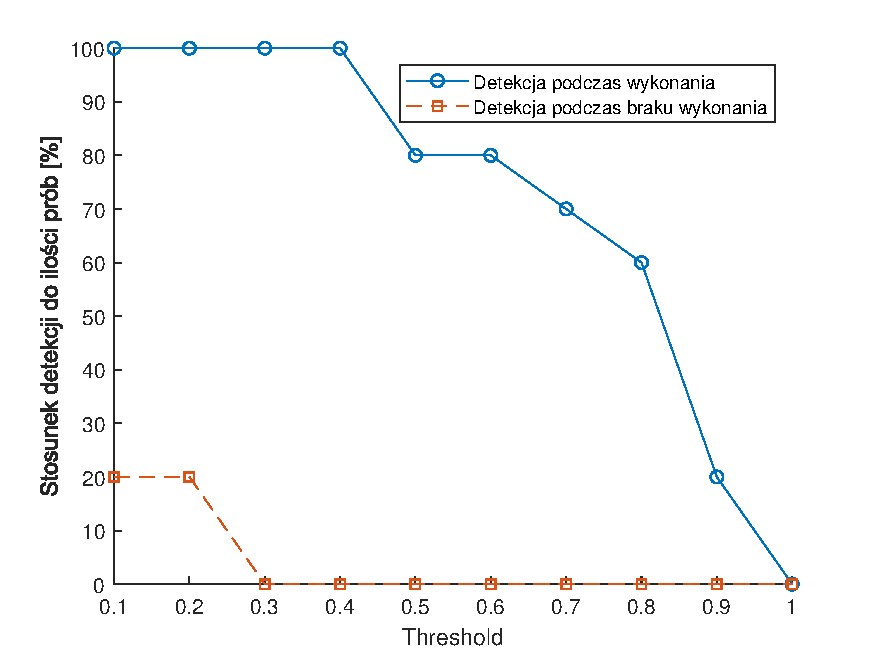
\includegraphics[width=\linewidth,keepaspectratio]{obrazy/frown1500}
    \caption{Zmarszczenie brwi, CFT = 1500 ms}
    \end{subfigure}\hspace*{\fill}
    \begin{subfigure}{0.3\linewidth}
    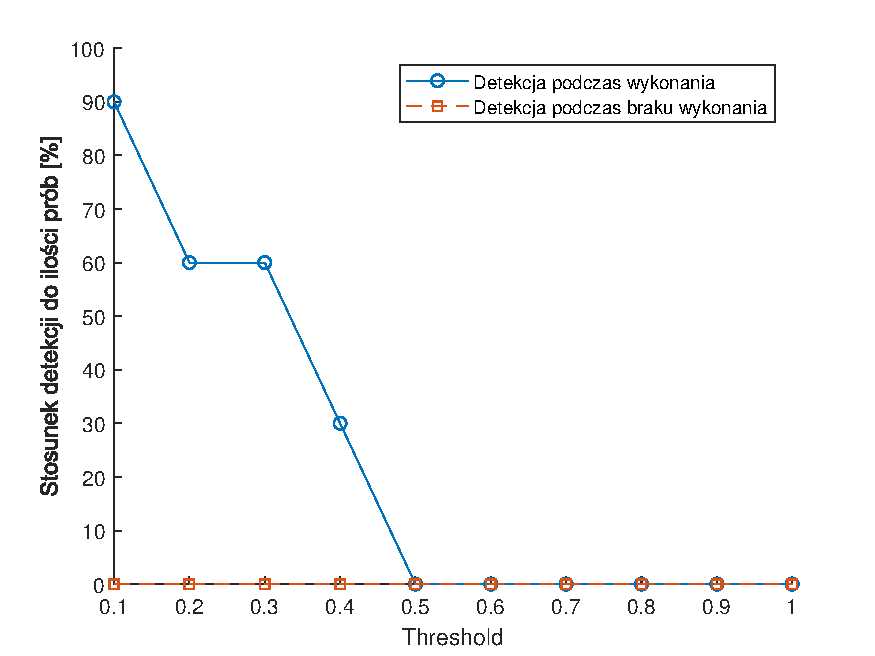
\includegraphics[width=\linewidth,keepaspectratio]{obrazy/frown2500}
    \caption{Zmarszczenie brwi, CFT = 2500 ms}
    \end{subfigure}
  \end{figure}
\end{frame}
\begin{frame}{Dodatkowe uwagi}
  \begin{columns}
    \begin{column}{0.5\textwidth}
      \begin{enumerate}[<+-|alert@+>]
        \item Wpływ zakłóceń\only<1>{: włosy, mimika, sieć}
        \item Ucisk urządzenia
        \item \textit{Reużywalność} treningu
      \end{enumerate}
    \end{column}
    \hfill
    \begin{column}{0.5\textwidth}
      \only<2>{
        \begin{figure}[htb]
          \centering
          \begin{subfigure}{\linewidth}
          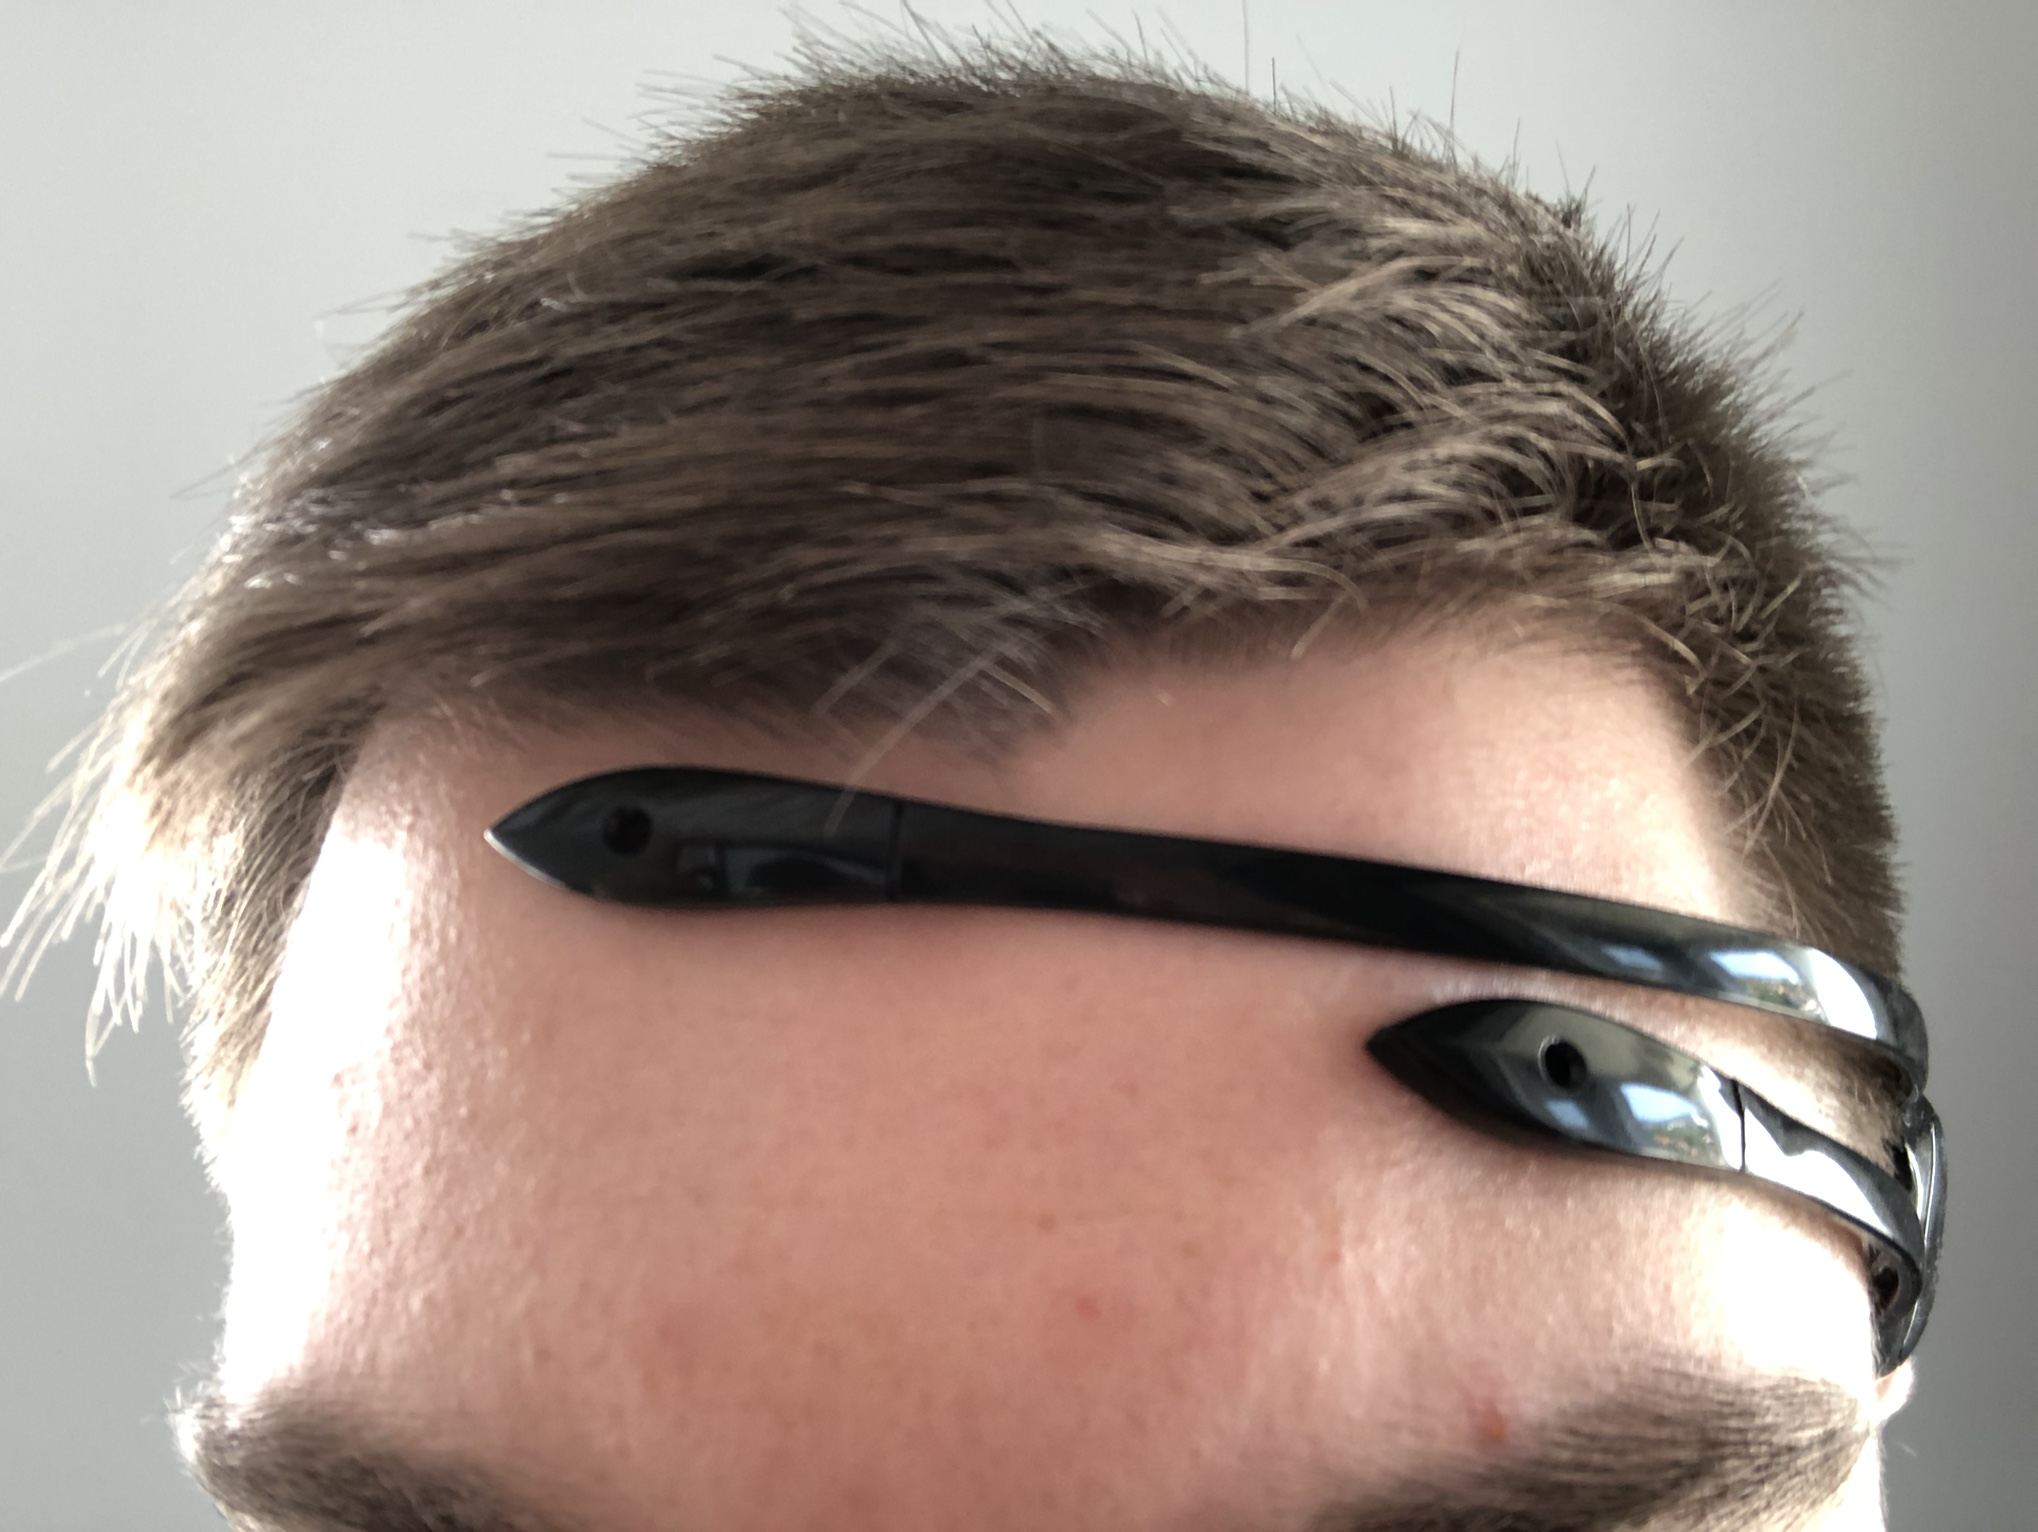
\includegraphics[width=\linewidth,height=0.4\textheight,keepaspectratio]{obrazy/headset_before}
          \end{subfigure}
          \par\medskip
          \begin{subfigure}{\linewidth}
          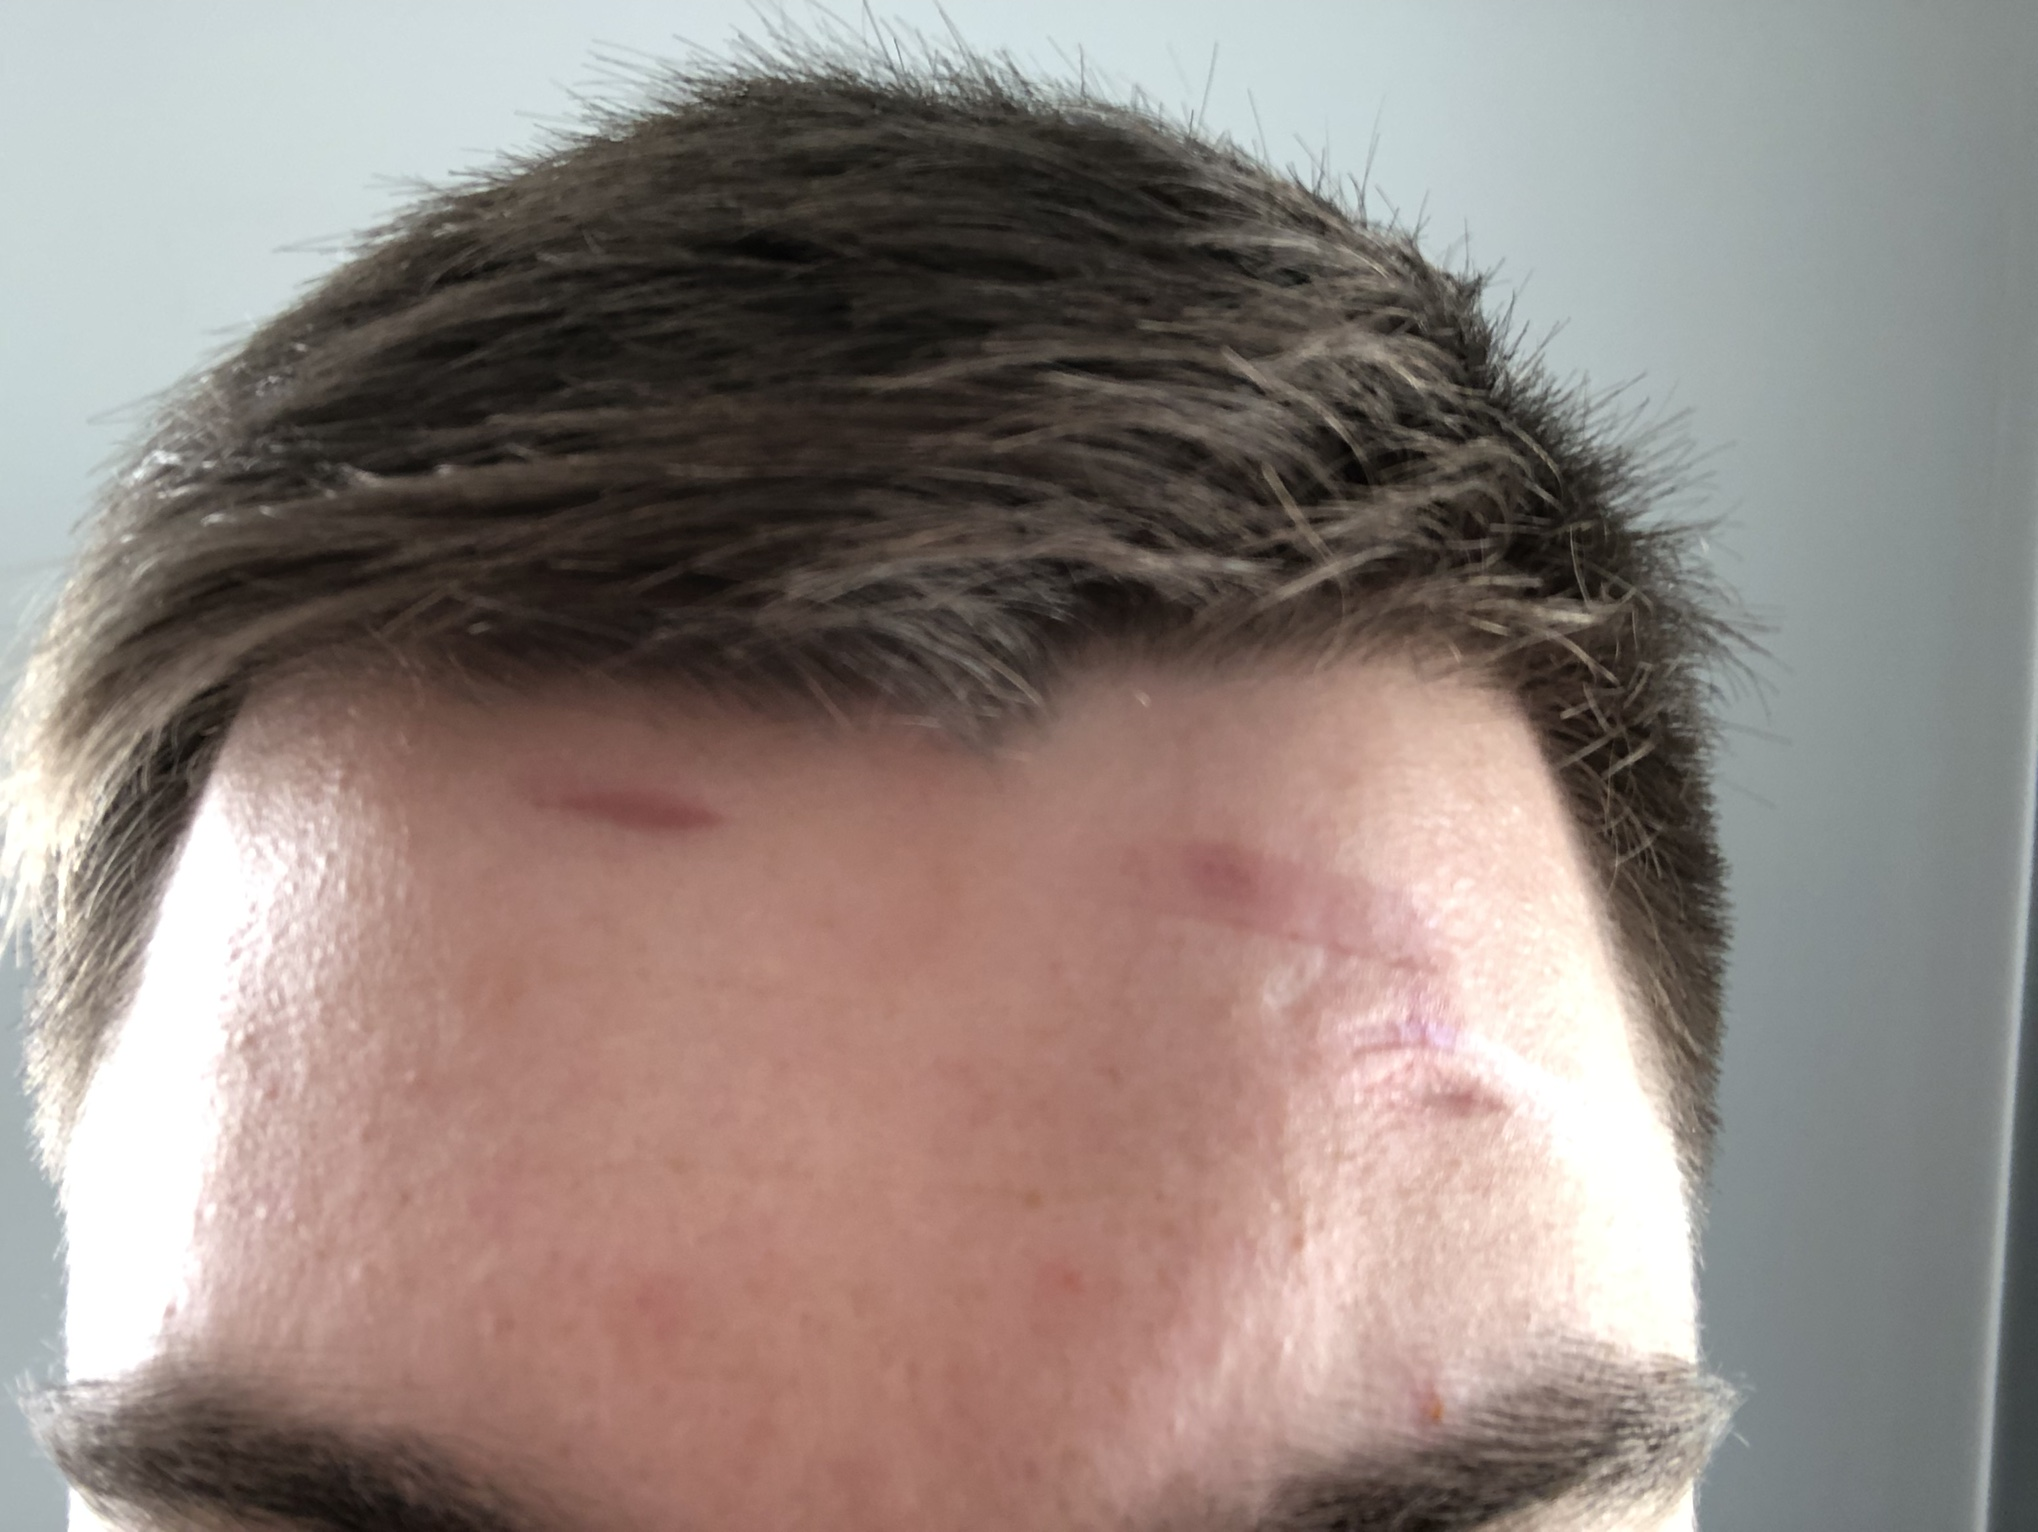
\includegraphics[width=\linewidth,height=0.4\textheight,keepaspectratio]{obrazy/headset_after}
          \end{subfigure}
        \end{figure}
      }
    \end{column}
  \end{columns}
\end{frame}

\section{Perspektywy dalszych usprawnień}

\begin{frame}{Perspektywy dalszych usprawnień}
  \begin{enumerate}[<+-|alert@+>]
    \item Dodanie obsługi dodatkowych urządzeń rejestrujących.
    \item Opracowanie algorytmu sterowania wykorzystującego wyłącznie detekcję mimiki.
    \item Usprawnienie klawiatury: podpowiedzi, autokorekta, wielojęzyczność, różne układy klawiszy.
  \end{enumerate}
\end{frame}

\begin{frame}[standout]
  Dziękuję za uwagę.
\end{frame}

\end{document}
